\begin{center}

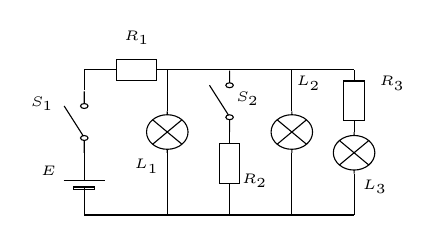
\begin{tikzpicture}[x=0.75pt,y=0.75pt,yscale=-1,xscale=1]
%uncomment if require: \path (0,300); %set diagram left start at 0, and has height of 300

%Shape: Battery [id:dp797984114545808] 
\draw   (100,170) -- (100,156.5) (90,153.5) -- (110,153.5) (100,153.5) -- (100,140) (95,157.7) -- (95,156.5) -- (105,156.5) -- (105,157.7) -- (95,157.7) -- cycle ;
%Shape: Simple Switch [id:dp4334800063265021] 
\draw   (100,140) -- (100,134.07) (100,116.29) -- (100,110.37) (99.39,131.7) -- (90.32,117.48) (100,118.66) .. controls (99,118.66) and (98.18,118.13) .. (98.18,117.48) .. controls (98.18,116.82) and (99,116.29) .. (100,116.29) .. controls (101,116.29) and (101.82,116.82) .. (101.82,117.48) .. controls (101.82,118.13) and (101,118.66) .. (100,118.66) -- cycle (100,134.07) .. controls (99,134.07) and (98.18,133.54) .. (98.18,132.89) .. controls (98.18,132.23) and (99,131.7) .. (100,131.7) .. controls (101,131.7) and (101.82,132.23) .. (101.82,132.89) .. controls (101.82,133.54) and (101,134.07) .. (100,134.07) -- cycle ;
%Shape: Resistor [id:dp901312688402967] 
\draw   (115.4,95) -- (134.6,95) -- (134.6,105) -- (115.4,105) -- (115.4,95) -- cycle (110,100) -- (115.4,100) (134.6,100) -- (140,100) ;
%Straight Lines [id:da2657385353492341] 
\draw    (100,110) -- (100,100) ;
%Straight Lines [id:da5416440059996896] 
\draw    (100,100) -- (110,100) ;
%Shape: Light Bulb [id:dp598022898779403] 
\draw   (140,138.33) .. controls (134.48,138.33) and (130,134.6) .. (130,130) .. controls (130,125.4) and (134.48,121.67) .. (140,121.67) .. controls (145.52,121.67) and (150,125.4) .. (150,130) .. controls (150,134.6) and (145.52,138.33) .. (140,138.33) -- cycle (132.88,135.93) -- (147.12,124.07) (132.88,124.07) -- (147.12,135.93) (140,140) -- (140,138.33) (140,121.67) -- (140,120) ;
%Straight Lines [id:da4277642056179305] 
\draw    (140,100) -- (140,120) ;
%Straight Lines [id:da9223803374157449] 
\draw    (100,170) -- (230,170) ;
%Straight Lines [id:da4800046187933087] 
\draw    (140,140) -- (140,170) ;
%Straight Lines [id:da5325118901733754] 
\draw    (140,100) -- (230,100) ;
%Shape: Light Bulb [id:dp8429011424978414] 
\draw   (200,138.33) .. controls (194.48,138.33) and (190,134.6) .. (190,130) .. controls (190,125.4) and (194.48,121.67) .. (200,121.67) .. controls (205.52,121.67) and (210,125.4) .. (210,130) .. controls (210,134.6) and (205.52,138.33) .. (200,138.33) -- cycle (192.88,135.93) -- (207.12,124.07) (192.88,124.07) -- (207.12,135.93) (200,140) -- (200,138.33) (200,121.67) -- (200,120) ;
%Straight Lines [id:da06826023906061329] 
\draw    (200,100) -- (200,120) ;
%Straight Lines [id:da15676855229008013] 
\draw    (200,140) -- (200,170) ;
%Shape: Simple Switch [id:dp5417474493250272] 
\draw   (170,130) -- (170,124.07) (170,106.29) -- (170,100.37) (169.39,121.7) -- (160.32,107.48) (170,108.66) .. controls (169,108.66) and (168.18,108.13) .. (168.18,107.48) .. controls (168.18,106.82) and (169,106.29) .. (170,106.29) .. controls (171,106.29) and (171.82,106.82) .. (171.82,107.48) .. controls (171.82,108.13) and (171,108.66) .. (170,108.66) -- cycle (170,124.07) .. controls (169,124.07) and (168.18,123.54) .. (168.18,122.89) .. controls (168.18,122.23) and (169,121.7) .. (170,121.7) .. controls (171,121.7) and (171.82,122.23) .. (171.82,122.89) .. controls (171.82,123.54) and (171,124.07) .. (170,124.07) -- cycle ;
%Shape: Resistor [id:dp5887325110380754] 
\draw   (165,154.6) -- (165,135.4) -- (175,135.4) -- (175,154.6) -- (165,154.6) -- cycle (170,160) -- (170,154.6) (170,135.4) -- (170,130) ;
%Straight Lines [id:da997349339495381] 
\draw    (170,160) -- (170,170) ;
%Straight Lines [id:da908902191522615] 
\draw    (230,150) -- (230,170) ;
%Shape: Light Bulb [id:dp15511171823131908] 
\draw   (230,148.33) .. controls (224.48,148.33) and (220,144.6) .. (220,140) .. controls (220,135.4) and (224.48,131.67) .. (230,131.67) .. controls (235.52,131.67) and (240,135.4) .. (240,140) .. controls (240,144.6) and (235.52,148.33) .. (230,148.33) -- cycle (222.88,145.93) -- (237.12,134.07) (222.88,134.07) -- (237.12,145.93) (230,150) -- (230,148.33) (230,131.67) -- (230,130) ;
%Shape: Resistor [id:dp2189689923867002] 
\draw   (225,124.6) -- (225,105.4) -- (235,105.4) -- (235,124.6) -- (225,124.6) -- cycle (230,130) -- (230,124.6) (230,105.4) -- (230,100) ;

% Text Node
\draw (78,145) node [anchor=north west][inner sep=0.75pt]  [font=\tiny] [align=left] {$\displaystyle E$};
% Text Node
\draw (73,112) node [anchor=north west][inner sep=0.75pt]  [font=\tiny] [align=left] {$\displaystyle S_{1}$};
% Text Node
\draw (172,109.29) node [anchor=north west][inner sep=0.75pt]  [font=\tiny] [align=left] {$\displaystyle S_{2}$};
% Text Node
\draw (118,80) node [anchor=north west][inner sep=0.75pt]  [font=\tiny] [align=left] {$\displaystyle R_{1}$};
% Text Node
\draw (174.8,148.8) node [anchor=north west][inner sep=0.75pt]  [font=\tiny] [align=left] {$\displaystyle R_{2}$};
% Text Node
\draw (241,102) node [anchor=north west][inner sep=0.75pt]  [font=\tiny] [align=left] {$\displaystyle R_{3}$};
% Text Node
\draw (123,142) node [anchor=north west][inner sep=0.75pt]  [font=\tiny] [align=left] {$\displaystyle L_{1}$};
% Text Node
\draw (201,102) node [anchor=north west][inner sep=0.75pt]  [font=\tiny] [align=left] {$\displaystyle L_{2}$};
% Text Node
\draw (233,152) node [anchor=north west][inner sep=0.75pt]  [font=\tiny] [align=left] {$\displaystyle L_{3}$};


\end{tikzpicture}

\end{center}